\documentclass[border=10pt]{standalone}

\usepackage{tikz}
\usepackage{tikzsymbols}
\usetikzlibrary{calc,patterns,shapes.geometric}

\def\centerarc[#1](#2)(#3:#4:#5){\draw[#1] ($(#2)+({#5*cos(#3)},{#5*sin(#3)})$) arc (#3:#4:#5);}

\begin{document}
	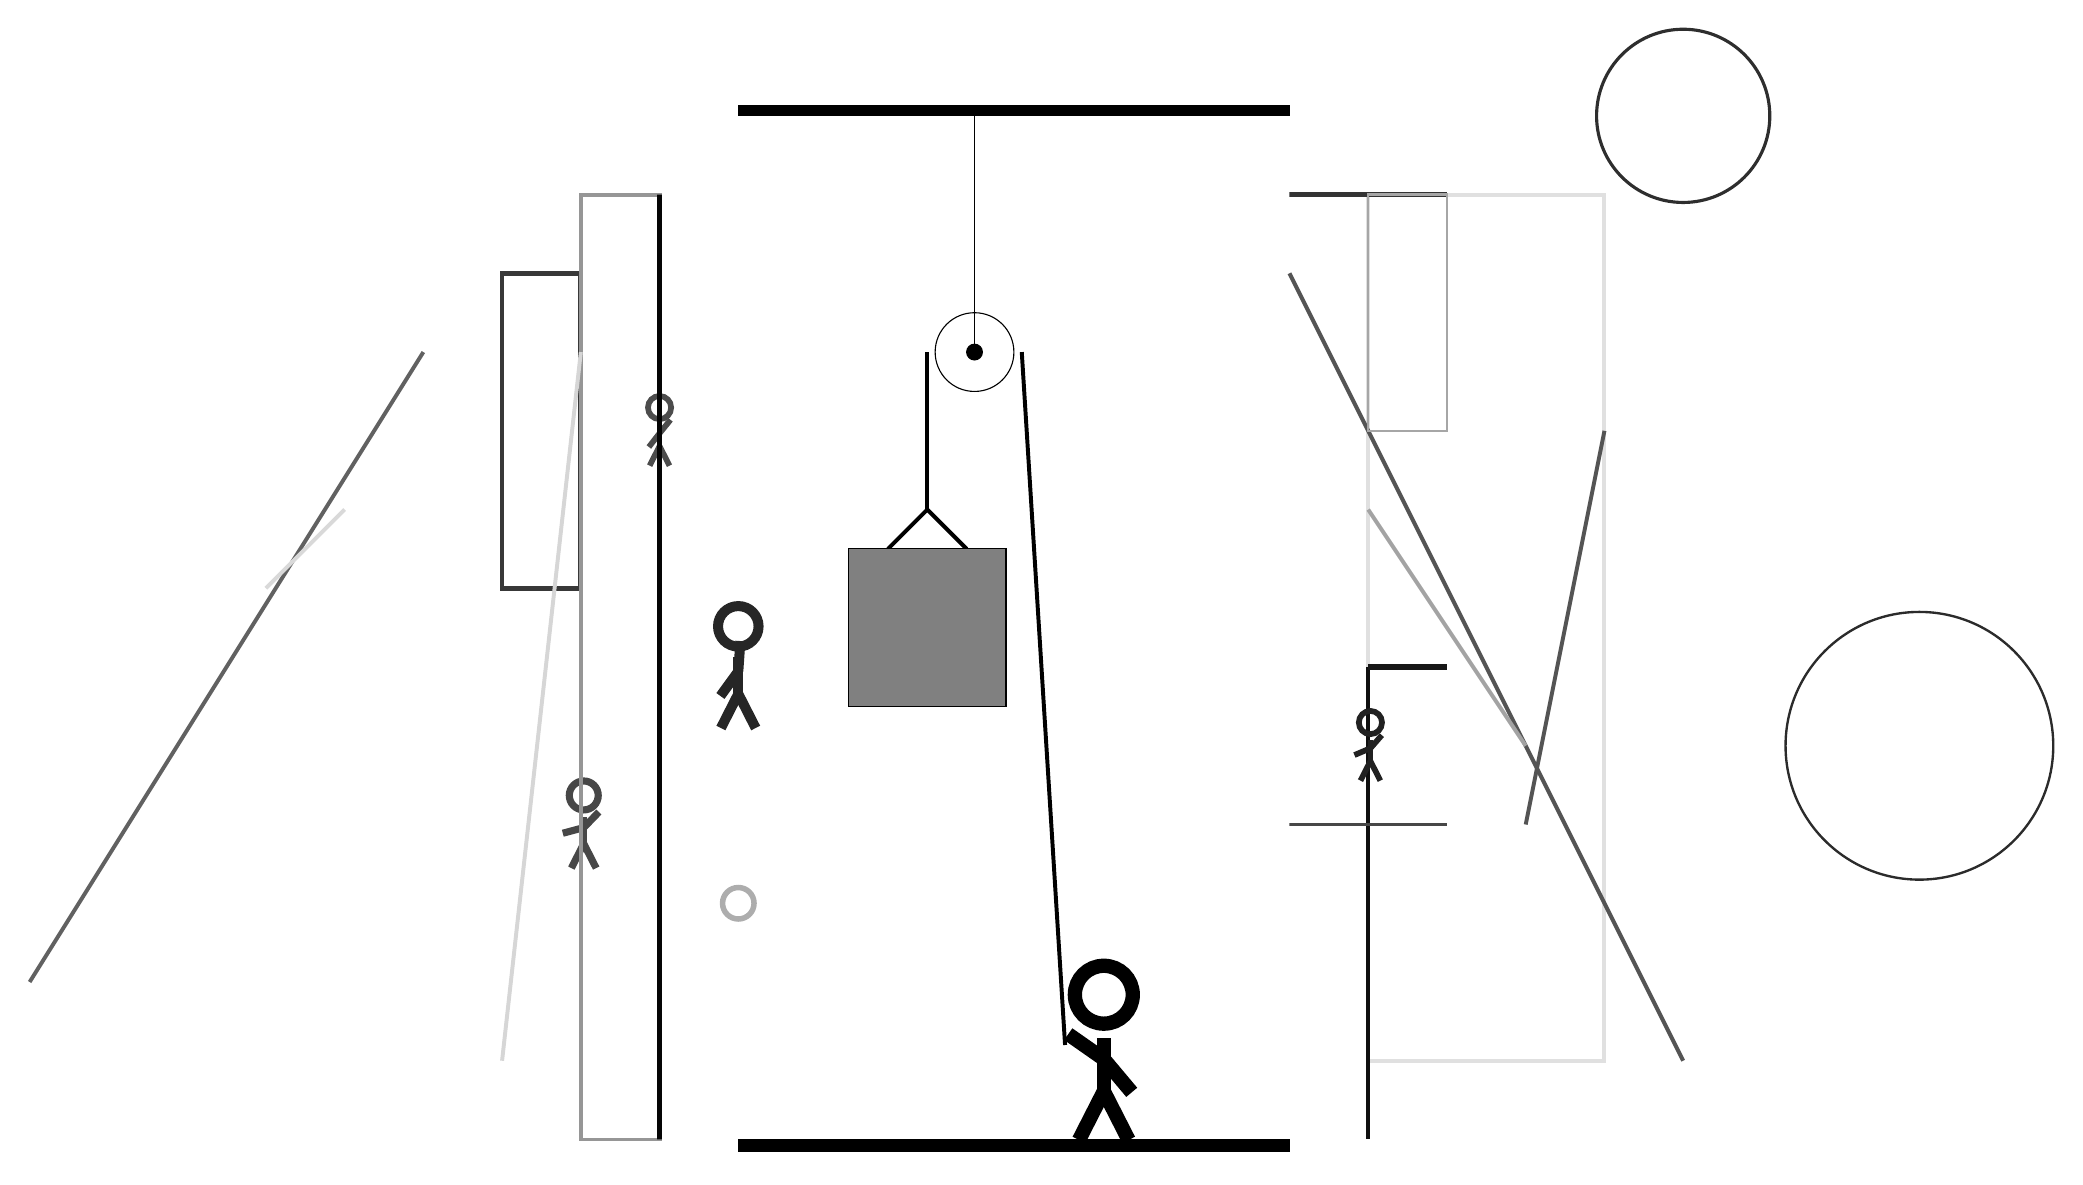
\begin{tikzpicture}
		%%%%% START %%%%%
		
		\draw[fill=black] (-2, 10) rectangle (5, 10.125);
		
		\draw[line width=0.6mm, color=black!78] (-4, 8) rectangle (-5, 4);
		
		\node[line width=0.3mm, color=black!70] at (-3, 6) {\Strichmaxerl[4][52][51]};
		\node[line width=0.2mm, color=black!72] at (-4, 1) {\Strichmaxerl[5][15][46]};
		\draw[line width=0.5mm, color=black!12] (6, 9) rectangle (9, -2);
		\node[line width=0.4mm, color=black!85] at (-2, 3) {\Strichmaxerl[7][54][86]};
		\draw[line width=0.5mm, color=black!94](6, 3) -- (6, -3);
		
		\draw[line width=0.7mm, color=black!91] (7, 3) rectangle (6, 3);
		
		\draw[line width=0.5mm, color=black!62](-6, 7) -- (-11, -1);
		\draw[line width=0.5mm, color=black!67](9, 6) -- (8, 1);
		\draw [line width=0.7mm, color=black!32](-2, 0) circle (0.2);
		
		\node[line width=0.7mm, color=black!87] at (6, 2) {\Strichmaxerl[4][23][49]};
		
		\draw [line width=0.4mm, color=black!82](10, 10) circle (1.1);
		\draw[line width=0.5mm, color=black!72] (5, 1) rectangle (7, 1);
		
		\draw[line width=0.5mm, color=black!15](-7, 5) -- (-8, 4);
		\draw[line width=0.5mm, color=black!41] (-3, -3) rectangle (-4, 9);
		\draw[line width=0.7mm, color=black!98] (-3, 9) rectangle (-3, -3);
		\draw[line width=0.7mm, color=black!80] (7, 9) rectangle (5, 9);
		\draw[line width=0.5mm, color=black!67](10, -2) -- (5, 8);
		\draw [line width=0.3mm, color=black!83](13, 2) circle (1.7);
		
		\draw[line width=0.3mm, color=black!35] (6, 6) rectangle (7, 9);
		\draw[line width=0.5mm, color=black!16](-4, 7) -- (-5, -2);
		
		\draw[line width=0.5mm, color=black!36](6, 5) -- (8, 2);
		
		\draw (1, 7) circle (0.5);
		\draw[fill=black] (1, 7) circle (0.1);
		\draw (1, 10) -- (1, 7);
		
		\draw[line width=0.5mm] (-0.1, 4.5) -- (0.4, 5.0) -- (0.9, 4.5);
		\draw[fill=black!50] (-0.6, 4.5) rectangle (1.4, 2.5);
		
		\draw[line width=0.5mm] (0.4, 7) -- (0.4, 5.0);
		\centerarc[line width=0.5mm](1, 7)(0:180:0.6);
		\draw[line width=0.5mm](1.6, 7) -- (2.15, -1.8);
		
		\node at (2.6, -1.9) {\Strichmaxerl[10][-35][-50]};
		
		\draw[fill=black] (-2, -3) rectangle (5, -3.15);
		
		%%%%% END %%%%%
	\end{tikzpicture}
\end{document}